% !TEX TS-program = pdflatex
% !TEX encoding = UTF-8 Unicode

% This is a simple template for a LaTeX document using the "article" class.
% See "book", "report", "letter" for other types of document.

\documentclass[11pt]{article} % use larger type; default would be 10pt

\usepackage[utf8]{inputenc} % set input encoding (not needed with XeLaTeX)

%%% Examples of Article customizations
% These packages are optional, depending whether you want the features they provide.
% See the LaTeX Companion or other references for full information.

%%% PAGE DIMENSIONS
\usepackage{geometry} % to change the page dimensions
\geometry{a4paper} % or letterpaper (US) or a5paper or....
% \geometry{margin=2in} % for example, change the margins to 2 inches all round
% \geometry{landscape} % set up the page for landscape
%   read geometry.pdf for detailed page layout information

\usepackage{graphicx} % support the \includegraphics command and options

% \usepackage[parfill]{parskip} % Activate to begin paragraphs with an empty line rather than an indent

%%% PACKAGES
\usepackage{booktabs} % for much better looking tables
\usepackage{array} % for better arrays (eg matrices) in maths
\usepackage{paralist} % very flexible & customisable lists (eg. enumerate/itemize, etc.)
\usepackage{verbatim} % adds environment for commenting out blocks of text & for better verbatim
\usepackage{subfig} % make it possible to include more than one captioned figure/table in a single float
% These packages are all incorporated in the memoir class to one degree or another...

%%% HEADERS & FOOTERS
\usepackage{fancyhdr} % This should be set AFTER setting up the page geometry
\pagestyle{fancy} % options: empty , plain , fancy
\renewcommand{\headrulewidth}{0pt} % customise the layout...
\lhead{}\chead{}\rhead{}
\lfoot{}\cfoot{\thepage}\rfoot{}

%%% SECTION TITLE APPEARANCE
\usepackage{sectsty}


\allsectionsfont{\sffamily\mdseries\upshape} % (See the fntguide.pdf for font help)
% (This matches ConTeXt defaults)

%%% ToC (table of contents) APPEARANCE
\usepackage[nottoc,notlof,notlot]{tocbibind} % Put the bibliography in the ToC
\usepackage[titles,subfigure]{tocloft} % Alter the style of the Table of Contents
\renewcommand{\cftsecfont}{\rmfamily\mdseries\upshape}
\renewcommand{\cftsecpagefont}{\rmfamily\mdseries\upshape} % No bold!

%%% END Article customizations


\usepackage[bulgarian]{babel}
\usepackage{physics}
\usepackage{amsmath}
\usepackage{centernot}
\usepackage{url}
\usepackage{graphicx}
\graphicspath{ {.} }
\usepackage{amsfonts}
\usepackage{xcolor}
\usepackage{enumitem}
\usepackage{systeme}


%%% The "real" document content comes below...

\title{23. Определен интеграл. Дефиниция и свойства. Интегруемост на непрекъснати функции...}
\author{Play4u}
%\date{} % Activate to display a given date or no date (if empty),
         % otherwise the current date is printed
         

\newcommand{\lrangle}[1]{\left\langle #1 \right\rangle}

\newcommand{\oversetModels}[1]{\overset{#1}{\models}}

\newcommand{\italicBold}[1]{\textbf{\emph{#1}}}

\newcommand{\definition}{\italicBold{Дефиниция: }}
\newcommand{\theorem}{\italicBold{Теорема: }}
\newcommand{\lemma}{\italicBold{Лема: }}
\newcommand{\proof}{\italicBold{Доказателство: }}
\newcommand{\statement}{\italicBold{Твърдение: }}
\newcommand{\source}{\italicBold{Източник: }}

\newcommand{\integral}[4]{\displaystyle \int_{#1}^{#2}#3\,#4}

\newcommand{\redText}[1]{\textcolor{red}{#1}}

\newcommand{\curlies}[1]{\{#1\}}
\newcommand{\overbar}[1]{\mkern 1.5mu\overline{\mkern-1.5mu#1\mkern-1.5mu}\mkern 1.5mu}

\newcommand{\enumNum}{\renewcommand{\theenumi}{\arabic{enumi}}}
\newcommand{\enumlet}{\renewcommand{\theenumi}{\alph{enumi}}} 

\begin{document}
\maketitle

\italicBold{Конспект: } Необходимо е да се докажат следните, формулирани общо, теореми: Нека $f$ е непрекъсната в затворения интервал $[a,b]$ и притежава производна поне в отворения интервал $(a,b)$. Да се докаже, че:

\enumlet
\begin{enumerate}
	\item ако $f(a)=f(b)$, то съществува такова $c \in (a,b)$, че $f'(c)=0$ (\textbf{Рол});\\
	\item съществува такова $c \in (a,b)$, че $f(b)-f(a)=f'(c)(b-a)$ (\textbf{Лагранж});\\
	\item ако $g$ е непрекъсната в затворения интервал $[a,b]$ и притежава производна поне в отворения интервал $(a,b), g'(x) \neq 0, x \in (a,b)$, то съществува такова $c \in (a,b)$, че \\
		\centerline{$\frac{f(b)-f(a)}{g(b)-g(a)}=\frac{f'(c)}{g'(c)} \qquad$ (\textbf{Коши}).}\\
\end{enumerate}
За доказателство на теоремата на Рол се иползва(\textit{без доказателство!}) теоремата на Вайерщрас, според която всяка непрекъсната функция в краен и затворен интервал достига своя максимум и минимум.\\
Необходимо е още да се изведе формулата на Тейлър с остатъчен член във формата на Лагранж.\\\par

Тези теореми играят основна роля за логическото изграждане на математическия анализ и за обосноваването на многобройните приложения на понятието производна.

\theorem \textbf{(1.)} Помощна теорема: Ако функцията $f$ има локален ексремум в точката $x_{0}$, то $f'(x_{0}) = 0$

\section{Теорема на Рол}
\theorem (\textbf{Рол: }) Нека функцията $f$ е дефинирана и непрекъсната в затворения интервал $[a,b]$ и диференцируема в отворения интервал $(a,b)$ и $f(a) = f(b)$. Тогава съществува такава точка $\xi \in (a,b): f'(\xi) = 0$.

Ще използваме теоремата на Вайерщрас, която гласи, че всяка непрекъсната функция върху краен затворен интервал достига своята най-голяма и най-малка стойност за някакви стойности принадлежащи на интервала. Т.е.\\
\centerline{$\exists x_{0}, x_{1} \in [a,b]:f(x_{1})=\underset{x \in [a,b]}{max} f(x); f(x_{0}) = \underset{x \in [a,b]}{min} f(x)$}
 Имаме следните възможности:\\

\enumNum
\begin{enumerate}
	\item функцията $f$ приема максималната или минималната си стойност в точка $\xi$, вътрешна за интервала $[a,b]$(т.е. $\xi \in [a,b]$). Тогава $f$ има локален екстремум в точката $\xi$ и $f'(\xi) = 0$ по теорема (\textbf{1.})\\
	\item функцията $f$ приема максималната и минималната си стойности в точка $a$ и $b$. Тогава от условието $f(a) = f(b)$ получаваме, че най-голямата и най-малката стойности на функцията $f$ съвпадат, следователно $f$ е константа и $f'(x)=0$ за всяко $x \in (a,b)$. С това теоремата е доказана\\\par
\end{enumerate}

\section{Теорема на Лагранж}
Следната теорема представлява един от най-често прилаганите резултати на диференциалното смятане:\par
\theorem (\textbf{за крайните нараствания, на Лагранж: }) Нека функцията $f$ е непрекъсната в затворения интервал $[a,b]$ и диференцируема в отворения интервал $(a,b)$. Тогава съществува такава точка $\xi \in (a,b)$, че \\
\centerline{$f(b)-f(a)=f'(\xi)(b-a) \qquad$ (формула за крайните нараствания)}
\par
\proof Разглеждаме функцията $h(x)=f(x)-kx$, където константата $k$ е подбрана така, че $h(a)=f(a)-ka=f(b)-kb=h(b)$, т.е. $k = \frac{f(b)-f(a)}{b-a}$. Очевидно функцията $h(x)$ удолетворява условията на теоремата на Рол, следователно съществува такава точка $\xi \in (a,b)$, че $h'(\xi)=f'(\xi)-k=0$. Оттук получаваме $k = \frac{f(b)-f(a)}{b-a} = f'(\xi)$, което доказва теоремата \\\par

\section{Теорема на Коши}
\theorem (\textbf{(Обобщена теорема  за крайните нараствания, или теорема на Коши: )} Нека функциите $f$ и $g$ са дефинирани и непрекъснати в затворения интервал $[a,b]$. Предполагаме, че $f(x)$ и $g(x)$ са диференцируеми в отворения интервал $(a,b)$ и $g'(x) \neq 0$ за всяко $x \in (a,b)$. Тогава съществува такава точка $\xi \in (a,b)$, че \\
\centerline{$\frac{f(b)-f(a)}{g(b)-g(a)}=\frac{f'(\xi)}{g'(\xi)}$}\\
\centerline{\textit{Обобщена формула за крайните нараствания}}
\par
\proof Прилагаме теоремата на Рол за функцията $h(x)=f(x)-kg(x)$, където константата $k$ е подбрана така, че $h(a) = f(a)-kg(a)=f(b)-kg(b)$, т.е. $k = \frac{f(b)-f(a)}{g(b)-g(a)}$. По теоремата на Рол съществува такава точка $\xi \in (a,b)$, че \\$h'(\xi)=f'(\xi)-kg'(\xi)=0$. Оттук получаваме, че\\
\centerline{$k = \frac{f(b)-f(a)}{g(b)-g(a)}=\frac{f'(\xi)}{g'(\xi)}$.} 


\section{формула на Тейлър с остатъчен член във формата на Лагранж}
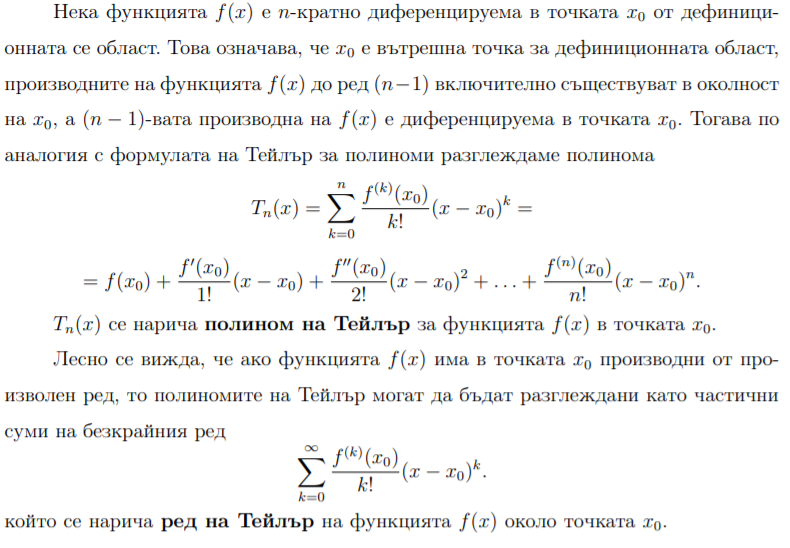
\includegraphics[scale=0.85]{Taylor1.png}\\
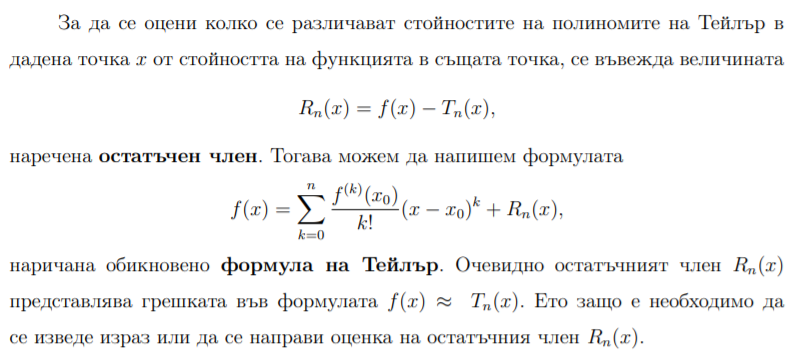
\includegraphics[scale=0.85]{Taylor2.png}\\
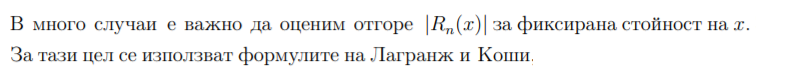
\includegraphics[scale=0.85]{Taylor3.png}\\
\textit{\textbf{Форма на Лагранж:}}\\
Нека функцията $f(x)$ притежава производни до ред $n+1$ включително в някаква околност на точката $a$ и $x$ е точка от тази околност. Тогава в интервала $(a,x)((x,a))$ съществува точка $\xi$, за която е в сила равенството \\
\centerline{$R_{n}(x) = \frac{f^{(n+1)}(\xi)}{(n+1)!}(x-a)^{n+1}$.}
\par
Това е най-често употребяваната форма на остатъчния член. При нея формулата на Тейлор добива вида:\\
\centerline{$f(x)=f(a)+\frac{f'(a)}{1!}(x-a)+...+\frac{f^{(n)}(a)}{n!}(x-a)^{n}+\frac{f^{n+1}(\xi)}{(n+1)!}(x-a)^{n+1}$.}
В частност при $n=0$ получаваме формулата \\
\centerline{$f(x)=f(a)+f'(\xi)(x-a)$.}
Прехвърлчйки $f(a)$ от лявата страна на равенството, виждаме, че показаната по-рано формула за крайните нараствания представлява частен случай на формулата на Тейлър.  

  
\end{document}





